\documentclass{beamer}
\usepackage{graphicx}
\usepackage{fancyvrb}
\usepackage{setspace,caption}
\usepackage{graphicx}
\usepackage{latexsym}
\usepackage{hyperref}
\usepackage[autostyle]{csquotes}

\setbeamertemplate{caption}[numbered]
\setbeamertemplate{theorems}[numbered]
\setbeamertemplate{navigation symbols}{}
\setbeamertemplate{bibliography item}{}
\setbeamertemplate{frametitle continuation}[from second]
\setbeamertemplate{footline}{
    \hfill
    \insertframenumber
    /
    \inserttotalframenumber
    \hspace{0.1cm}
}

\hypersetup{
  colorlinks = true,
  linkcolor = blue
}
\makeatletter
\let\@mycite\@cite
\def\@cite#1#2{{\hypersetup{linkcolor=green!60!black}[{#1\if@tempswa , #2\fi}]}}
\makeatother



\usepackage{xcolor}
\def\HiLi{\leavevmode\rlap{\hbox to \hsize{\color{yellow}\leaders\hrule height .8\baselineskip depth .5ex\hfill}}}
\def\HiLo{\leavevmode\rlap{\hbox to \hsize{\color{yellow}\leaders\hrule height 1.5\baselineskip depth 2.5ex\hfill}}}
\def\HiLa{\leavevmode\rlap{\hbox to \hsize{\color{yellow}\leaders\hrule height 1\baselineskip depth 0.8ex\hfill}}}

\usepackage{color, colortbl}


\AtBeginSection[] {
\begin{frame}<beamer>
\frametitle{Outline} 
\begin{scriptsize}
\tableofcontents[currentsection]  
\end{scriptsize}
\end{frame}
}

\bibliographystyle{apalike}
\newcommand\Fontvi{\fontsize{9}{7.2}\selectfont}



\begin{document}
%%%%%%%%%%%%%%%%%%%%%%%%%%%%%%%%%%%%%%%%%%%%%%%%%%%%%%%%%%%%%%%%%%%%%%%%%%%%%%%%%%%%%%%%%%%%%%%%%%%%%%%%%%%%%%%%%%%%%%%%%%%%%%%%%%%%%%%%%%%%%%%%%%%%%%
\begin{frame}
    \title{\bf Example of a beamer presentation}
    \author{Ricardo Pontaza}
    \date{\today}
    \titlepage
\end{frame}
%%%%%%%%%%%%%%%%%%%%%%%%%%%%%%%%%%%%%%%%%%%%%%%%%%%%%%%%%%%%%%%%%%%%%%%%%%%%%%%%%%%%%%%%%%%%%%%%%%%%%%%%%%%%%%%%%%%%%%%%%%%%%%%%%%%%%%%%%%%%%%%%%%%%%%

\section{First section}
\begin{frame}
\frametitle{First slide}
This is an example of a slide.
\end{frame}

\begin{frame}
\frametitle{First slide}
This is an example of a slide.

If you want to add extra slides, just use the the \textbf{frame} environment, with the \textbf{frametitle} command to input your title.
\end{frame}


\section{Second section}
\subsection{Subsection}
\begin{frame}
\frametitle{How to add elements}
You can use any \emph{align, enumerate, equation, array} environment, just add their respective packages.
\end{frame}

\section{Bibliography}
\begin{frame}
\frametitle{Bibliography}
In order to have a bibliography, modify the .bib file in this project. For example, let's suppose you want to add an specific book in your references:
\begin{enumerate}
\item Look the book/paper/publication in Google scholar.
\item Next to the match found, there is a \emph{cite} link. Click on it.
\item At the bottom, there is the \textbf{Bibtex} style. Click on it.
\item Copy the citation into your .bib file.
\item Run BibTeX on your file to make the linkage to your text. 
\end{enumerate}
\end{frame}

\begin{frame}
\frametitle{Bibliography}
\begin{figure}
  \centering
  % Requires \usepackage{graphicx}
  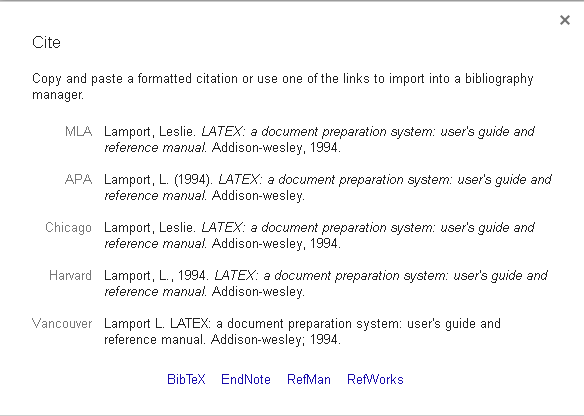
\includegraphics[width=8cm]{bibtex1.png}\\
  \caption{Image of how to get a good BibTeX citation.}\label{BibTeX_citation}
\end{figure}
\end{frame}



\section{References}
\begin{frame}[allowframebreaks]
\frametitle{References}
\nocite{*}
\Fontvi\bibliography{references}
\end{frame}

\end{document}
\begin{frame}
\begin{center}
Demo
\end{center}
\end{frame}



\begin{frame}
\frametitle{}

\end{frame}

$\mathbb{F}_{q^{k}}$
